\chapter{Outline}
\label{chp:out}

\section{The big picture}
\begin{figure}[tp]
  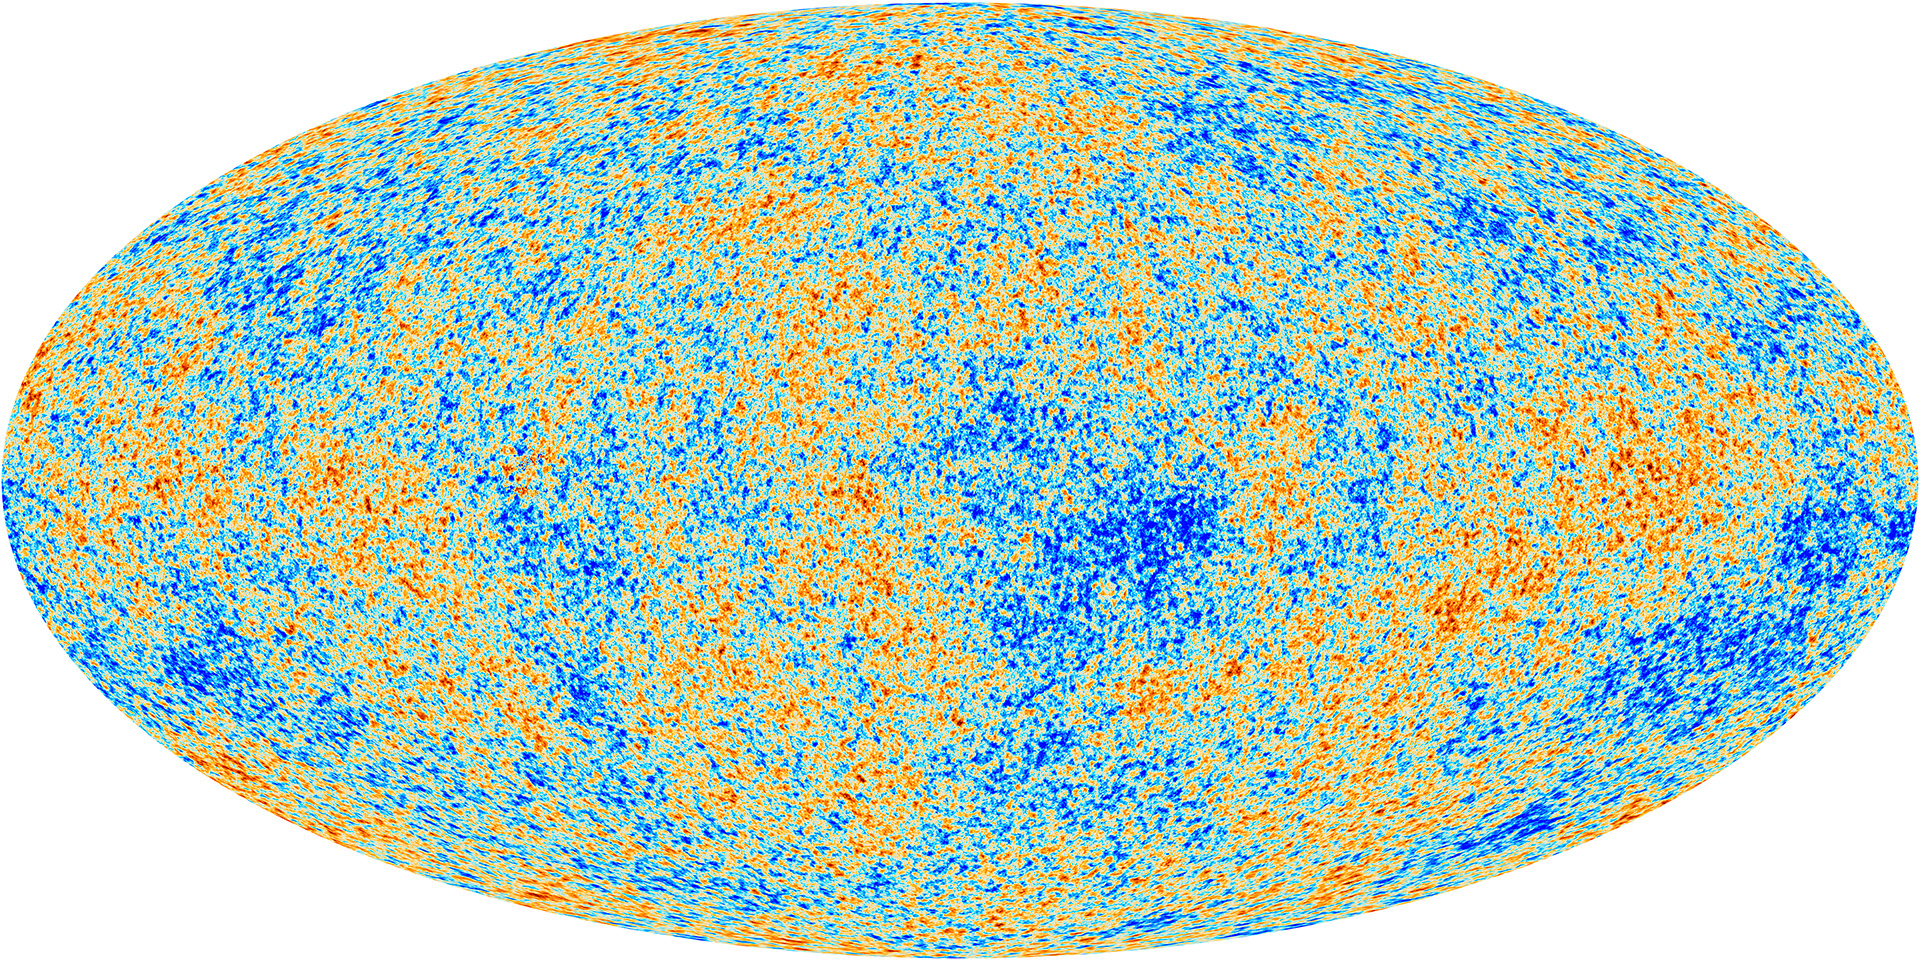
\includegraphics[width=\textwidth]{chapters/outline/figures/planck}
  \caption{Temperature distortions in the cosmic microwave background.}\label{fig:out:planck}
\end{figure}

As cosmologists, nature has been incredibly kind to us. We have been given a near crystal clear snapshot of the universe a mere \(380,000\) years after its birth. Maps created by the Planck satellite (Figure~\ref{fig:out:planck}) allow us to determine the patterns of density in the early universe. For cosmologists these density distortions are interesting in two ways. 

First, these perturbations in density are the beginnings of the formation of stars, galaxies and galaxy clusters. If one were to wind the clock forwards from this moment, cosmic structure would be seen coalescing around the regions of higher density.

Second, these distortions tell us a great deal about physics at much earlier times. Observations from particle physics experiments allow us to confidently wind the clock backwards to mere microseconds after the big bang.
However, the expansion of the universe itself allows us to look even further back than this. We now have a wealth of observational evidence that early in its history, the universe underwent a rapid accelerated expansion. This expansion acts as a cosmic magnifying glass, allowing us to observe patterns \(\sim10^{-32}\) seconds after the big bang using the universe we see today. The upshot of this is that cosmologists effectively have access to the most powerful particle accelerator imaginable, reaching energies trillions of times greater than the Large Hadron Collider. 

The canonical explanation for the early period of accelerated expansion is the theory of inflation, with quantum fields providing the necessary driving force. This thesis focusses on the initial conditions for inflation; i.e.\ what started this all off.

\section{Kinetic initial conditions}

Traditionally, cosmologists work under the assumption that at these early times the universe was in an effectively eternal inflating state, with no detectable beginning. Chapter~\ref{chp:kd} rigorously proves a result that suggests this picture may be somewhat incomplete. In fact, almost all classical universes begin at a finite time in the past. Moreover, this beginning is dominated by kinetic energy, and not inflating. This provides a novel and arguably simpler mechanism for setting the initial conditions of the universe. More importantly, I also show that this period could have produced a distinct observational signature in the primordial power spectrum of curvature perturbations. Chapter~\ref{chp:kt} details how this mathematical observation fits into more traditional approaches.

As a member of the Planck collaboration, I began to search for evidence of this pre-inflationary phase. Chapter~\ref{chp:rec} details a model-independent reconstruction of the primordial spectrum. Whilst not conclusive, there are tantalising hints of a signal consistent with a pre-inflationary epoch.

\section{Observations in high dimensions}
\begin{figure}[tp]
  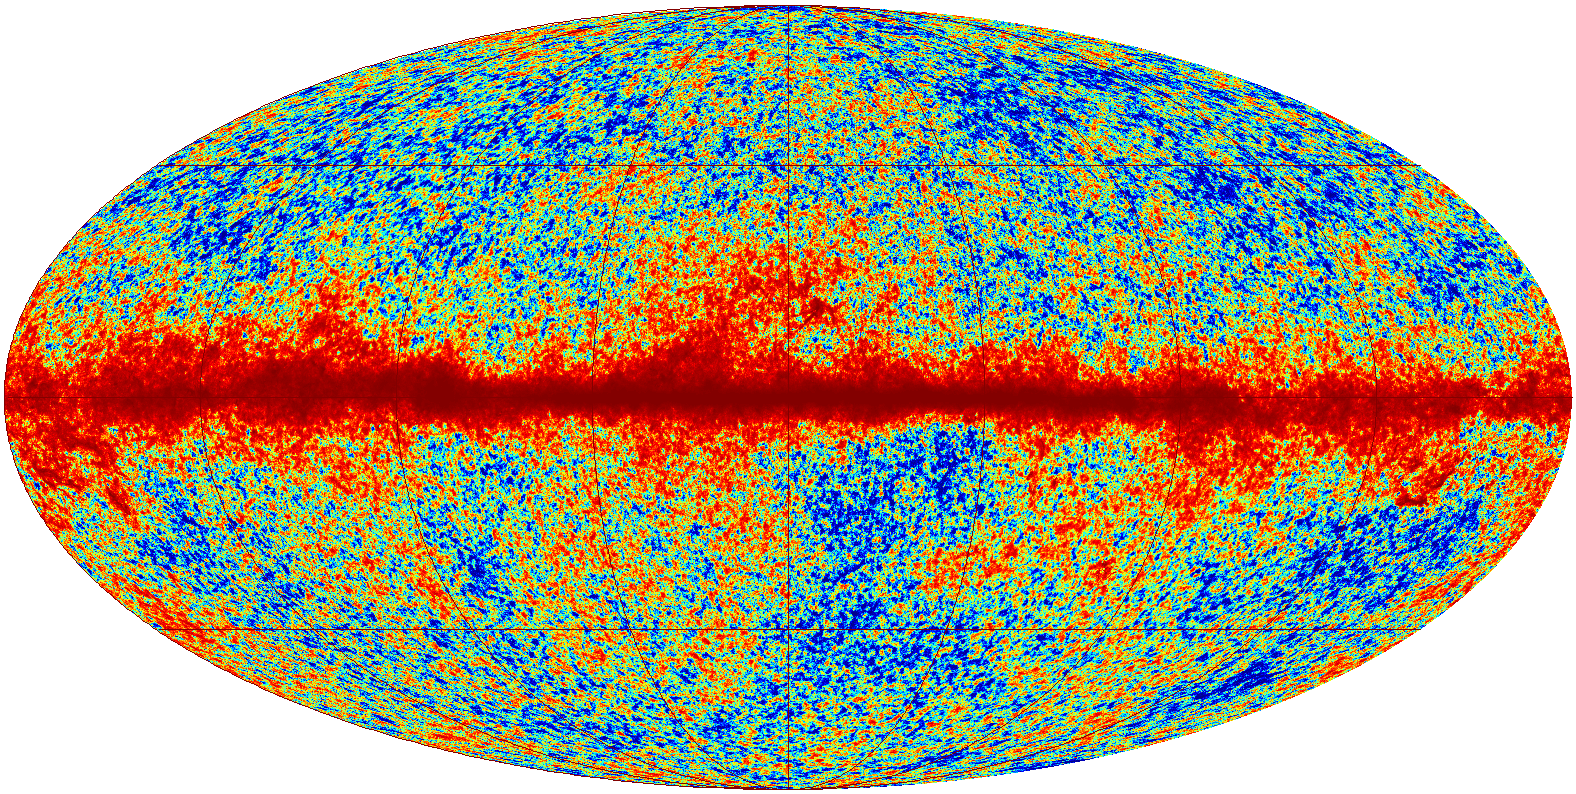
\includegraphics[width=\textwidth]{chapters/outline/figures/planck_galaxy}
  \caption{The microwave sky as seen by Planck at 143GHz.}\label{fig:out:planck_galaxy}
\end{figure}
Our microwave sky does not look like Figure~\ref{fig:out:planck}. The sky that Planck actually sees is more akin to Figure~\ref{fig:out:planck_galaxy}. The most notable difference between the two figures is the presence of a red band in the centre of the second image, which are the microwaves emitted by our own Milky Way galaxy. In order to observe the signal generated by the beginning of the universe (Figure~\ref{fig:out:planck}), we must first take into account the contaminating information of the Milky Way. This requires a sophisticated model of the galaxy, with many parameters that must be simultaneously determined and quantified. 

Whilst attempting to reconstruct the primordial power spectrum (Chapter~\ref{chp:rec}), it became apparent that there was an absence of Bayesian data analysis tools. The techniques available at the time were incapable of navigating and integrating the complicated high-dimensional likelihoods required for my reconstruction.

The Cavendish Astrophysics group has a long history of developing and applying novel Bayesian statistical approaches. With this in mind, I designed and implemented a novel nested sampling algorithm which was christened PolyChord (detailed in Chapter~\ref{chp:pc}). This proved capable of scaling to the dimensionalities required, and reliably computing  the Bayesian evidence, allowing me to produce model-independent reconstructions of the primordial power spectrum.
As a result, PolyChord was rapidly adopted by many members of the team as their de-facto inference tool.

\section{Quantum initial conditions}
My latest work focusses on the quantum mechanical initial conditions of the early universe. A full theoretical treatment of this epoch requires a consideration of quantum fields in curved spacetime. One of the critical issues of this field is that the basic concepts we use to describe quantum particles are not designed to work in the context of gravity as a curved spacetime background. My latest research aims to resolve some of these issues, by building the quantum vacuum around the renormalised stress energy tensor. In essence, I hypothesise that empty space could be better defined as ``lowest energy'' rather than ``particle-less''. I also demonstrated that in the context of the early universe this alternative viewpoint makes detectable predictions which again differ from standard theory. This is detailed in Chapter~\ref{chp:qv}.

Whilst examining this, I realised that I needed a better way of solving the differential equations of the early universe. I succeeded in developing a novel class of extremely efficient numerical methods for solving these, which I term Runge-Kutta-Wentzel-Kramers-Brillouin approaches. RKWKB is explained Chapter~\ref{chp:RK}.

\section{Thesis versus research}
\begin{figure}[tp]
  \centering
  \tikzsetnextfilename{sequence}
  %\tikzset{external/export next=false}

\begin{tikzpicture}[%
    node distance = 5mm,
    writing/.style={%
      text width=30mm,  % default text width
      align=center      % align in center
    },
    component/.style={%
      writing,          % writing style above
    },
    connection/.style={%
      very thick,      % very thick arrows
      >=stealth        % pretty arrow head
    }
]

  \node[component] (KD) at (0,0) {Kinetic dominance\\(Chapter~\protect\ref{chp:kd})};

  \node[below left = of KD, component] (TO)  {Theoretical observations\\(Chapter~\protect\ref{chp:kt})};

  \node[below = of KD, component] (PS) {Power spectrum reconstruction\\(Chapter~\protect\ref{chp:rec})};

  \node[right = of PS, component] (NS) {Nested sampling\\(Chapter~\protect\ref{chp:ens})};

  \node[below = of NS, component] (PC) {\PolyChord{}\\(Chapter~\protect\ref{chp:pc})};

  \node[below = of TO, component] (RE) {Quantum\\ kinetic dominance\\(Chapter~\protect\ref{chp:qv})};

  \node[below = of RE, component] (RK) {RKWKB\\(Chapter~\protect\ref{chp:RK})};

  \node[right = of RK, component] (FUT) {Constraining the kinetically dominated universe\\(Future research)};

    \draw[connection,->] (KD) -- (PS);
    \draw[connection,->] (KD) -- (TO);
    \draw[connection,->] (NS) -- (PC);
    \draw[connection,->] (PC) -- (PS);
    \draw[connection,->] (TO) -- (RE);
    \draw[connection,->] (PS) -- (RE);
    \draw[connection,->] (RE) -- (RK);
    \draw[connection,->] (RE) -- (FUT);
    \draw[connection,->] (PC) -- (FUT);
    \draw[connection,->] (RK) -- (FUT);
    \draw[connection,->] (PS) -- (FUT);

\end{tikzpicture}

  \includegraphics[width=\textwidth]{chapters/outline/plots/sequence.tikz}
  \caption{The ``sequence'' of my research.}\label{fig:out:sequence}
\end{figure}

The theme of this thesis is the interplay between theory, observations and methods. Whilst the thesis divided into two parts, in reality both halves have strongly influenced each other in a manner not necessarily consistent with the sequence of the text. Figure~\ref{fig:out:sequence} shows an approximate set of interactions between the various chapters. Whilst a thesis must be laid out sequentially, actual research is often very non-linear. The degree committee requires that a dissertation be a ``connected account of research'', and whilst this thesis is not sequentially connected, it does at least form a directed acyclic graph.
